\section{Example Using Two Quadrilaterals}
\label{sec:example:twoquad4}

PyLith features discussed in this example:
\begin{itemize}
\item Quasi-static solution
\item Mesh ASCII format
\item Dirichlet boundary conditions
\item Neumann boundary conditions
\item Kinematic fault interface conditions
\item Plane strain linearly elastic material
\item VTK output
\item Bilinear quadrilateral cells
\item SimpleDB spatial database
\item ZeroDispDB spatial database
\end{itemize}
All of the files necessary to run the examples are contained in the
directory \filename{examples/twocells/twoquad4.}


\subsection{Overview}

This example is another simple 2D example of a quasi-static finite
element problem. It is a mesh composed of two bilinear quadrilaterals
subject to displacement or traction boundary conditions, assuming
plane-strain linear elastic behavior. Due to the simple geometry of
the problem, the mesh may be constructed by hand, using PyLith mesh
ASCII format to describe the mesh. In this example, we will walk
through the steps necessary to construct, run, and view four problems
that use the same mesh. In addition to this manual, each of the files
for the example problem includes extensive comments.


\subsection{Mesh Description}

The mesh consists of two square cells with edge lengths of one unit
forming a regular region (Figure \vref{fig:twoquad4-mesh}). The mesh
geometry and topology are described in the file \filename{twoquad4.mesh},
which is in PyLith mesh ASCII format. This file describes the dimensionality
of the problem (in this case 2D), the coordinates of the vertices
(nodes), the vertices composing each cell (element), the material
ID to be associated with each cell, and then provides groups of vertices
that may be used to define faults or surfaces to which boundary conditions
may be applied.

\begin{figure}
  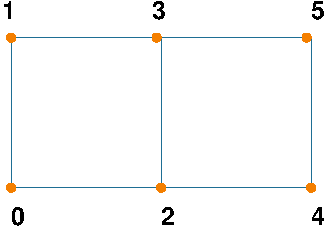
\includegraphics{examples/figs/twoquad4-mesh}
  \caption{Mesh composed of two bilinear quadrilateral cells used for
    the example problems.}
  \label{fig:twoquad4-mesh}
\end{figure}


\subsection{Additional Common Information}

In addition to the mesh, the four example problems share additional
information. As in the previous examples, we place this information
in \filename{pylithapp.cfg}, since this file is read automatically every
time PyLith is run. Settings specific to a particular problem may
be placed in other \filename{cfg} files, as described later, and then
those files are placed on the command line.


\subsection{Axial Displacement Example}

The first example problem is extension of the mesh along the x axis.
Parameter settings that override or augment those in \filename{pylithapp.cfg}
are contained in the file \filename{axialdisp.cfg}. These include:
\begin{inventory}
  \facilityitem{pylithapp.timedependent.bc.x\_neg}{Specifies the
    boundary conditions for the left side of the mesh, defining which
    degrees of freedom are being constrained (x), giving the label
    (defined in \filename{twoquad4.mesh}) defining the points desired,
    assigning a label to the boundary condition set, and giving the
    name of the spatial database with the values for the Dirichlet
    boundary condition (\filename{axialdisp.spatialdb}).}
  \facilityitem{pylithapp.timedependent.bc.x\_pos}{Specifies the
    boundary conditions for the right side of the mesh, defining which
    degrees of freedom are being constrained (x), giving the label
    (defined in \filename{twoquad4.mesh}) defining the points desired,
    assigning a label to the boundary condition set, and giving the
    name of the spatial database defining the boundary conditions
    (\filename{axialdisp.spatialdb}).}
  \facilityitem{pylithapp.timedependent.bc.y\_neg}{Specifies the
    boundary conditions for the bottom two corners of the mesh,
    defining which degrees of freedom are being constrained (y),
    giving the label (defined in \filename{twoquad4.mesh}) defining
    the points desired, assigning a label to the boundary condition
    set, and giving the name of the spatial database with the values
    for the Dirichlet boundary condition
    (\filename{axialdisp.spatialdb}).}
\end{inventory}
The values for the Dirichlet boundary condition are given in the file
\filename{axialdisp.spatialdb}, as specified in
\filename{axialdisp.cfg}.  Because the data are being specified using
two control points with a linear variation in the values between the
two (rather than being uniform over the mesh, for example), the data
dimension is one.

The files containing common information (\filename{twoquad4.mesh},
\filename{pylithapp.cfg}, \filename{matprops.spatialdb}) along with
the problem-specific files (\filename{axialdisp.cfg},
\filename{axialdisp.spatialdb}) provide a complete description of the
problem, and we can then run this example by typing
\begin{shell}
$ pylith axialdisp.cfg
\end{shell}
As in the two triangle axial displacement example, three files will be
produced. If the problem ran correctly, you should be able to produce
a figure such as Figure \vref{fig:twoquad4-axial}, which was generated
using ParaView.

\begin{figure}[htbp]
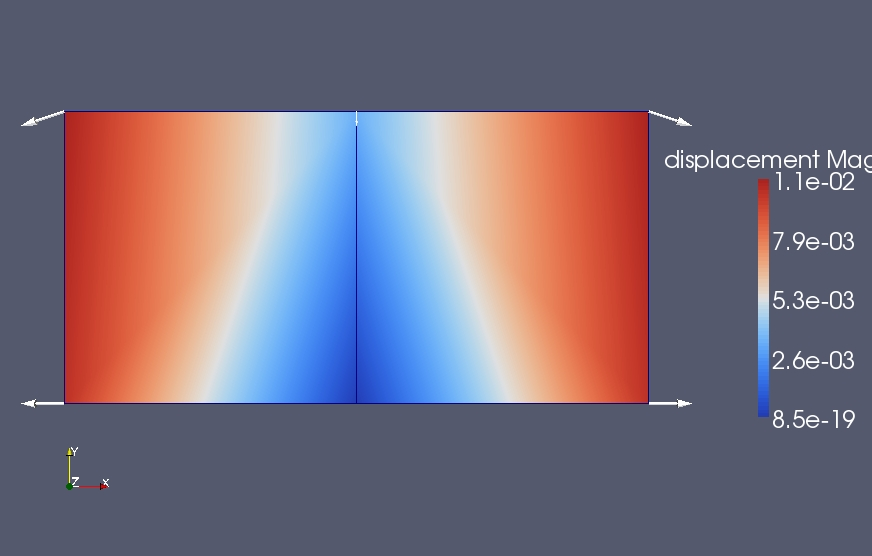
\includegraphics[scale=0.33]{examples/figs/twoquad4-axialdisp}
\caption{Color contours and vectors of displacement for the axial displacement
  example using a mesh composed of two bilinear quadrilateral cells.}
\label{fig:twoquad4-axial}
\end{figure}


\subsection{Shear Displacement Example}

The next example problem is shearing of the mesh in the y direction
using displacements applied along the positive and negative x
boundaries.  Parameter settings that override or augment those in
\filename{pylithapp.cfg} are contained in the file
\filename{sheardisp.cfg}. These include:
\begin{inventory}
  \facilityitem{pylithapp.timedependent.bc.x\_neg}{Specifies the
    boundary conditions for the left side of the mesh, defining which
    degrees of freedom are being constrained (x and y), giving the
    label (\facility{x\_neg}, defined in \filename{twoquad4.mesh})
    defining the points desired, assigning a label to the boundary
    condition set, and giving the name of the spatial database with
    the values for the Dirichlet boundary condition
    (\filename{sheardisp.spatialdb}).}
  \facilityitem{pylithapp.timedependent.bc.x\_pos}{Specifies the
    boundary conditions for the left side of the mesh, defining which
    degrees of freedom are being constrained (y only), giving the
    label (\facility{x\_pos}, defined in \filename{twoquad4.mesh})
    defining the points desired, assigning a label to the boundary
    condition set, and giving the name of the spatial database with
    the values for the Dirichlet boundary condition
    (\filename{sheardisp.spatialdb}).}
\end{inventory}
The values for the Dirichlet boundary conditions are described in the
file \filename{sheardisp.spatialdb}, as specified in
\filename{sheardisp.cfg}.  In this case, the desired displacement
values are given at two control points, corresponding to the two edges
we want to constrain. Since data are being specified at two points
with a linear variations in the values between the points (rather than
being uniform over the mesh, for example), the data dimension is one.

The files containing common information (\filename{twoquad4.mesh},
\filename{pylithapp.cfg}, \filename{matprops.spatialdb}) along with
the problem-specific files (\filename{sheardisp.cfg},
\filename{sheardisp.spatialdb}) provide a complete description of the
problem, and we can then run this example by typing
\begin{shell}
$ pylith sheardisp.cfg
\end{shell}
As in the previous example, three files will be produced. If the
problem ran correctly, you should be able to produce a figure such as
Figure \vref{fig:twoquad4-shear}, which was generated using ParaView.

\begin{figure}
  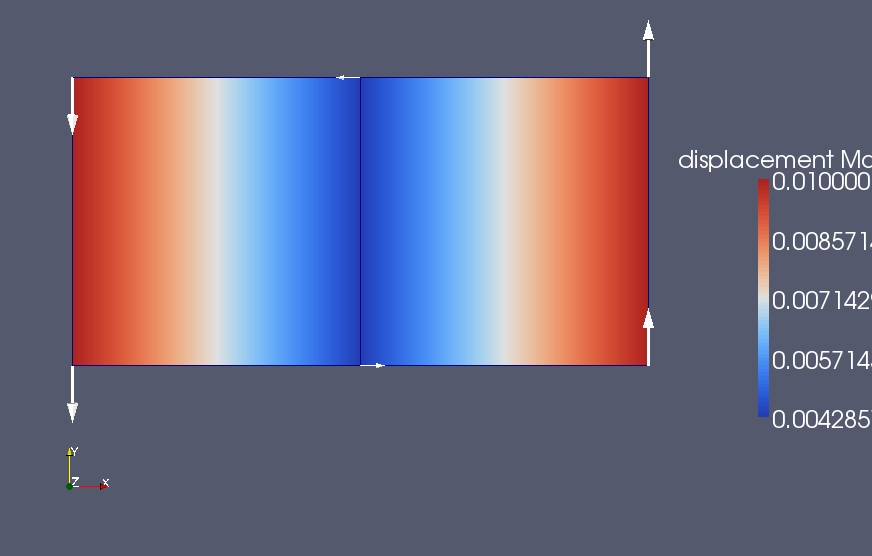
\includegraphics[scale=0.33]{examples/figs/twoquad4-sheardisp}
  \caption{Color contours and vectors of displacement for the shear
    displacement example using a mesh composed of two bilinear
    quadrilateral cells.}
  \label{fig:twoquad4-shear}
\end{figure}


\subsection{Kinematic Fault Slip Example}

The next example problem is a left-lateral fault slip applied between
the two square cells using kinematic cohesive cells. The left and
right boundaries are held fixed in the x and y directions. Parameter
settings that override or augment those in \filename{pylithapp.cfg}
are contained in the file \filename{dislocation.cfg}. These settings
include:
\begin{inventory}
\facilityitem{pylithapp.timedependent.bc.x\_neg}{Specifies the
  boundary conditions for the left side of the mesh, defining which
  degrees of freedom are being constrained (x and y), giving the label
  (\facility{x\_neg}, defined in \filename{twoquad4.mesh}) defining
  the points desired, and assigning a label to the boundary condition
  set. Instead of specifying a spatial database file for the values of
  the Dirichlet boundary condition, we use the default spatial
  database (ZeroDispDB) for the Dirichlet boundary condition, which
  sets the displacements to zero for all time.}
\facilityitem{pylithapp.timedependent.bc.x\_pos}{Specifies the
  boundary conditions for the right side of the mesh, defining which
  degrees of freedom are being constrained (x and y), giving the
  label (\facility{x\_neg}, defined in \filename{twoquad4.mesh})
  defining the points desired, and assigning a label to the boundary
  condition set. We use the ZeroDispDB for this boundary condition
  as well, which sets the displacements to zero for all time.}
\facilityitem{pylithapp.timedependent.interfaces}{Gives the label
  (defined in \filename{twoquad4.mesh}) defining the points on the
  fault, provides quadrature information, and then gives database
  names for material properties (needed for conditioning), fault
  slip, peak fault slip rate, and fault slip time.}
\end{inventory}
The fault example requires three additional database files that were
not needed for the simple displacement examples. The first file
(\filename{dislocation\_slip.spatialdb}) specifies 0.01 m of
left-lateral fault slip for the entire fault.  The data dimension is
zero since the same data are applied to all points in the set. The
default slip time function is a step-function, so we also must provide
the time at which slip begins. The elastic solution is associated with
advancing from $t=-dt$ to $t=0$, so we set the slip initiation time
for the step-function to 0 in
\filename{dislocation\_sliptime.spatialdb}.

The files containing common information (\filename{twoquad4.mesh},
\filename{pylithapp.cfg}, \filename{matprops.spatialdb}) along with
the problem-specific files (\filename{dislocation.cfg},
\filename{dislocation\_slip.spatialdb},
\filename{dislocation\_sliptime.spatialdb}) provide a complete
description of the problem, and we can then run this example by typing
\begin{shell}
$ pylith dislocation.cfg
\end{shell}
The addition of a fault results in two additional output files (as in
the two triangle fault example),
\filename{dislocation-fault\_t0000000.vtk} and
\filename{dislocation-fault\_info.vtk}.  These files provide output of
fault slip, change in tractions, and diagnostic information such as
the normal direction, final slip, and slip time for each vertex on the
fault. If the problem ran correctly, you should be able to produce a
figure such as Figure \vref{fig:twoquad4-disloc}, which was generated
using ParaView.

\begin{figure}
  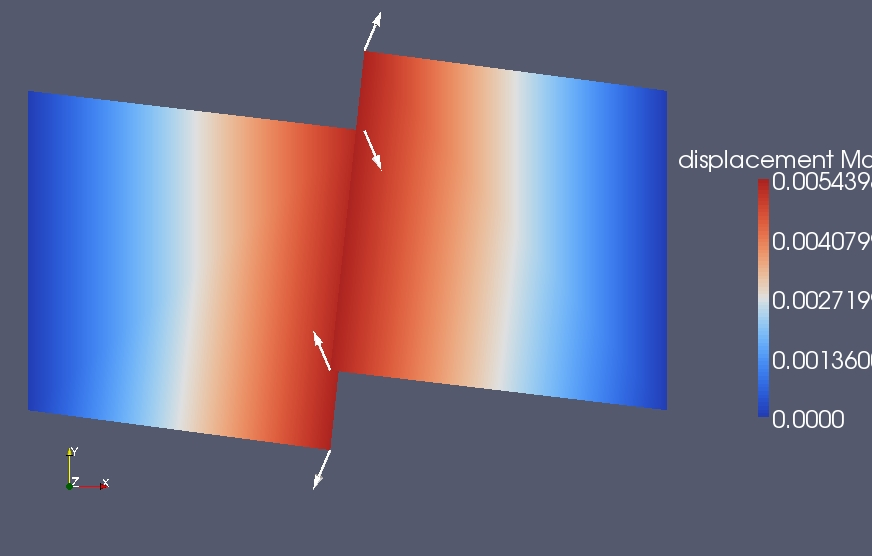
\includegraphics[scale=0.33]{examples/figs/twoquad4-dislocation}
  \caption{Color contours and vectors of displacement for the kinematic fault
    example using a mesh composed of two bilinear quadrilateral cells.}
  \label{fig:twoquad4-disloc}
\end{figure}


\subsection{Axial Traction Example}
\label{sec:examples:twoquad4-traction}

The fourth example demonstrates the use of Neumann (traction) boundary
conditions. Constant tractions are applied to the right edge of the
mesh, while displacements normal to the boundaries are held fixed
along the left and bottom edges of the mesh. Parameter settings that
override or augment those in \filename{pylithapp.cfg} are contained
in the file \filename{axialtract.cfg}. These settings include:
\begin{inventory}
\facilityitem{pylithapp.timedependent}{Specifies an implicit
  formulation for the problem and specifies the array of boundary
  conditions. The boundary condition type for \facility{x\_pos} is
  explicitly set to \object{Neumann}, since the default boundary
  condition type is \object{DirichletBC}.}
\facilityitem{pylithapp.timedependent.bc.x\_neg}{Specifies the
  boundary conditions for the left side of the mesh, defining which
  degrees of freedom are being constrained (x) and giving the label
  (defined in \filename{twoquad4.mesh}) defining the points
  desired. In this case, rather than specifying a spatial database
  file with values for the Dirichlet boundary conditions, we use the
  default spatial database (ZeroDispDB) for the Dirichlet boundary
  condition, which sets the displacements to zero for all time.}
\facilityitem{pylithapp.timedependent.bc.x\_pos}{Specifies the
  Neumann boundary conditions for the right side of the mesh,
  giving the label (defined in \filename{twoquad4.mesh}) defining
  the points desired, assigning a label to the boundary condition
  set, and giving the name of the spatial database with the
  traction vectors for the Neumann boundary condition
  (\filename{axialtract.spatialdb}).}
\facilityitem{pylithapp.timedependent.bc.y\_neg}{Specifies the
  boundary conditions for the bottom two corners of the mesh,
  defining which degrees of freedom are being constrained (y)
  and giving the label (defined in \filename{twoquad4.mesh})
  defining the points desired. In this case, we again use the
  ZeroDispDB, which sets the displacements to zero for all time.}
\facilityitem{pylithapp.problem.formulation.output.output.writer}{Gives
  the base filename for VTK output (\filename{axialtract.vtk}).}
\facilityitem{pylithapp.timedependent.bc.x\_pos.output}{Gives
  the field to be output for the \facility{x\_pos} boundary
  (\texttt{tractions}), and gives the base filename for
  \facility{x\_pos} boundary output
  (\filename{axialtract-tractions.vtk}).}
\end{inventory}
The traction vectors for the Neumann boundary conditions are given in
the file \filename{axialtract.spatialdb}, as specified in
\filename{axialtract.cfg}.  The files containing common information
(\filename{twoquad4.mesh}, \filename{pylithapp.cfg},
\filename{matprops.spatialdb}) along with the problem-specific files
(\filename{axialtract.cfg}, \filename{axialtract.spatialdb}) provide a
complete description of the problem, and we can then run this example
by typing
\begin{shell}
$ pylith axialtract.cfg
\end{shell}
Once the problem has run, six files will be produced. This includes
the five files as in the previous example plus
\filename{axialtract-tractions\_info.vtk}, which gives the \texttt{x}
and \texttt{y} components of traction applied at each integration
point. If the problem ran correctly, you should be able to produce a
figure such as Figure \vref{fig:twoquad4-axialtract}, which was
generated using ParaView. The results may be compared against the
analytical solution derived in Section
\vref{sub:Analytical-Constant-Traction}.

\begin{figure}
  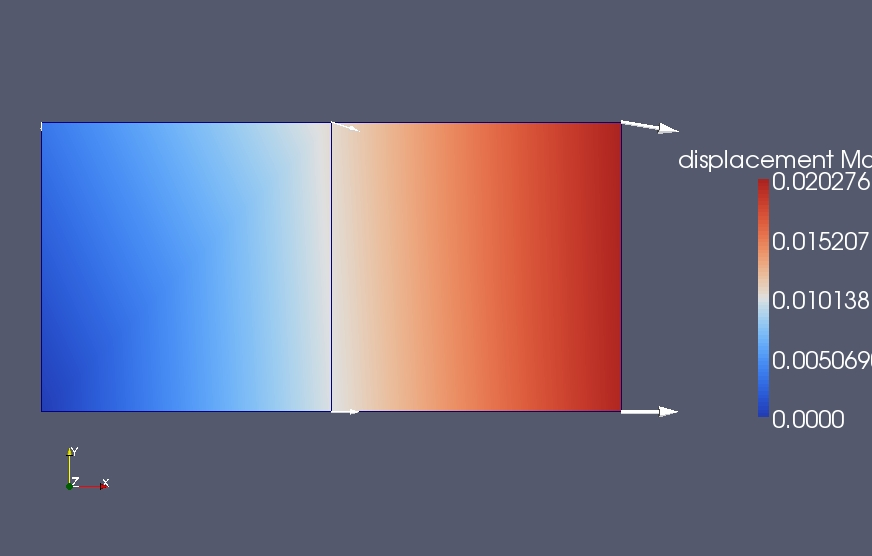
\includegraphics[scale=0.33]{examples/figs/twoquad4-axialtract}
  \caption{Color contours and vectors of displacement for the axial traction
    example using a mesh composed of two bilinear quadrilateral cells.}
  \label{fig:twoquad4-axialtract}
\end{figure}


% End of file
